\section{Muon / Tail Catcher Detector}
Most recent update: 2018-06-04 \\
Contact person: Valeri Saveliev (email : saveliev@mail.desy.de)

%%%%%%%%%%%%%%%%%%%%%%%%%%%%%%%%%%%%%
\subsection{Introduction}
The main goals of the Muon System for the ILC Detector are the identification and reconstruction of the muons from inelastic $\Pep\Pem$ interactions over the largest possible energy and angular range and recovery of the energy leakage out of the hadron calorimeter (Energy Tail Catcher).
The physics goals set for the ILD detector require that muons momentum are reconstructed with high precision of about $\Delta p_T/p^2_T = 2 \times10^{-5}$.
Due to the large amount of material muons have to traverse before reaching the muon detection system, it cannot provide the required momentum resolution and will be optimized mainly to the high efficiency and purity of muon identification.
A momentum resolution of the required precision has to be achieved with by the tracking system. An important aspect is the efficient linking of track candidates from the inner detectors with tracks in the muon detection system.
In addition to its muon identification ability, the first layers of the muon detection system will be optimized to act as a tail catcher for showers developing late in the calorimeters. This will improve the energy measurement in the hadron calorimeter, especially for the highest energies.
Another aspect of the muon system is the stand-alone identification and reconstruction of beam-halo muons. This requirement has an impact on the muon system granularity and time resolution, which shall be better than \SI{1}{ns}.

%%%%%%%%%%%%%%%%%%%%%%%%%%%%%%%%%%%%%%
\subsection{Conceptual Design of the Muon/Tail Catcher Detection System}
Important constraints for the design of the muon detection system at ILC as for many other experiments is the instrumentation of the detection elements inside the Iron return yoke, needed for the magnetic flux return of the detector solenoid.
The Muon/Tail Catcher Detection System instruments the Iron return yoke in the barrel and in the forward regions with maximal coverage.
The needed mechanical stability requires that the Iron return yoke layer thickness is at least \SI{10}{cm}. The muon detectors will be interleaved between such iron plates, which are used as absorbers.
The requirement that the Muon/Tail Catcher Detection System serves both as a muon identifier and as a tail catcher impacts its layout design.
The first section of the system provides ten relatively closely spaced layers, to act as a continuation of the hadron calorimeter.
As mentioned above the mechanical constraints limit the absorber thickness to be at least \SI{10}{cm}.
At the rear of the muon system the distance between stations can be increased, since they are only needed for the muon identification and reconstruction.
The last three layers in the barrel, and two in the end cap are spaced \SI{60}{cm} apart.
The fact that the solenoid magnet coil adds about two interaction lengths of material in front of the muon detection system limits the effect of the tail catcher.
To maximize its impact the first sensitive layer is placed in front of the iron yoke, directly behind the coil and the first 10 layers are spaced more closely to improve the calorimetric performance of the muon system.
The Iron yoke barrel part is equipped with one sensitive layer in front of the iron yoke, 10 layers spaced \SI{14}{cm} apart, followed by three sensitive layers spaced by \SI{60}{cm} apart. The overall layout of the muon /tail catcher system is shown in Figure~\ref{fig:ild:muon:tailCatcher}.
\begin{figure}
	\centering
	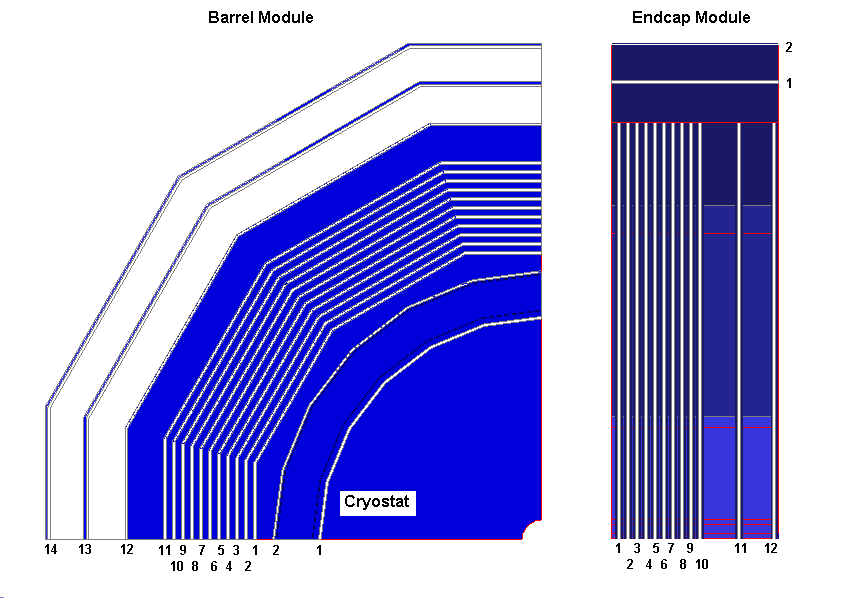
\includegraphics[height=8cm]{MuonDetector/MuonDetectorILD/2D_barel_endcap.png}
	\caption{Sensitive Layers of ILD Muon /Tail Catcher Detector}
	\label{fig:ild:muon:tailCatcher}
\end{figure}

Two main options are investigated for the muon detection elements: scintillator strips equipped with wave-length shifting fibers and readout with silicon photomultipliers (Sc/SiPM), or pixelated gas detectors - resistive plate chambers (RPC).

%%%%%%%%%%%%%%%%%%%%%%%%%%%%%%%%%%%%
\section{Scintillator/Silicon Photomultiplier}
Most recent update: 2017-02-25 \\
Contact person: Valeri Saveliev (email : saveliev@mail.desy.de )

\subsection{Introduction}
The main option for the sensitive layers will use extruded plastic scintillation strips, composed of polystyrene doped with 1.0\% PPO and 0.03\% POPOP.
The extruded scintillator has a width of \SIrange{25}{30}{mm} and thickness of \SI{10}{mm}.

A \SI{1}{mm} wide extruded groove running along the centre of the strip will take a commercially available wave length shifting (WLS) fibers.
The groove is filled with a white epoxy made of DER 332 resin and Jeffamine.

The scintillator strips will be covered on the outside by a layer of \ce{TiO2}, that is co-extruded with the scintillator strips during the extrusion process.

The maximal length of strips required for ILD is \SI{250}{cm}.

The signals will be readout from both sides of the strips by Silicon Photomultipliers, coupled to the WLS fibres.
Reading out both sides of a strip offers the possibility to define the position of the hits along the strip, which will help in reducing the fake rate in the muon detection system.

Figure~\ref{fig:ild:muon:concept} (top) shows the design of the scintillator strip. The bottom picture presents the signal (number of photons) of the scintillation strip with WLS and SiPM readout from both sides.

\begin{figure}
	\centering
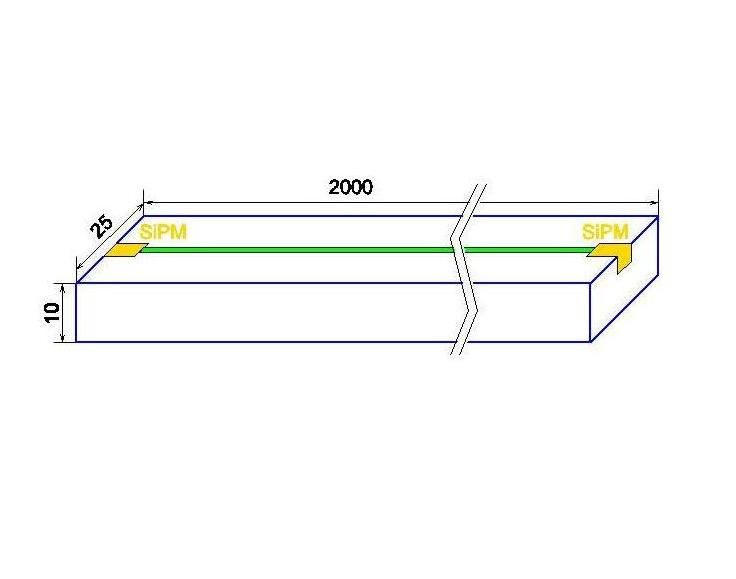
\includegraphics[height=8cm]{MuonDetector/MuonDetectorILD/Sc_strip.jpg}
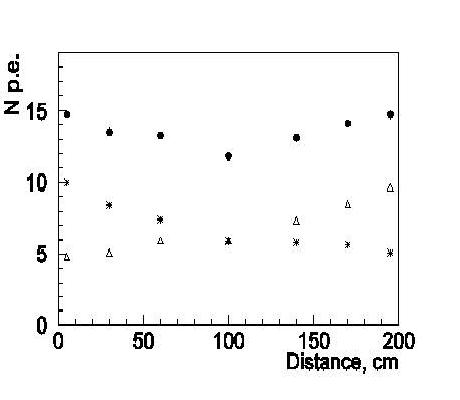
\includegraphics[height=8cm]{MuonDetector/MuonDetectorILD/Sc_strip_photons.jpg}
	\caption{Sensitive Layers of ILD Muon/Tail Catcher Detector and number of detected photons as a function of distance}
	\label{fig:ild:muon:concept}
\end{figure}

%%%%%%%%%%%%%%%%%%%%%%%%%%%%%%%%%%%%
\subsection{Recent Milestones}
The major R\&D effort of the Muon/Tail Catcher Detection System development was concentrated on the optimization of the overall structure of the Muon/Tail Catcher System:
\begin{enumerate}
\item Detailed Monte Carlo Simulation of the Muon/Tail Catcher System, performed to choose the geometry of detection plane, geometry of the stereo layers, number of the layers of the detection system and their position, especially concerning the energy leakage.
\item Study of the performance of the Muon/Tail Catcher System with framework of Partice Flow Algorithm (PFA).
\item Optimization of the detection elements of the Muon/Tail Catcher System. The first priority is the design of the main detection elements a scintillation strips with the SiPM readout.
\item Development of the digital options of the SiPM for the Muon/Tail Catcher System, which will dramatically simplify the readout electronics and data processing.
\end{enumerate}

%%%%%%%%%%%%%%%%%%%%%%%%%%%%%%%%%%%%
\subsection{Engineering Challenges}
The main engineering challenge is the distributed large scale of the Muon/Tail Catcher System and its embedded in the solenoid magnet yoke.
Several layouts for the muon system have been investigated.

\subsection{Future Plans}
Continued optimization of the Muon/Tail Catcher Detection System using the detailed Monte Carlo simulation and reconstruction framework.
\begin{itemize}
\item The performance of the muon system has been evaluated by simulating events in the ILD concept. To determine the optimal layout,
a geometry was created in MOKKA with 14 layers in the barrel and 12 layers in the end cap, first eleven layers at equal distances of \SI{140}{mm} and distances of \SI{640}{mm} of last three layers in the barel and first ten layers at equal distances of \SI{140}{mm} and of last three layers at equal distances of \SI{640}{mm} in the end cap . After simulating the detector response in MOKKA, different layouts could be studied by including or excluding layers at the reconstruction phase. For this study the muon layers have been segmented in pads of $30\times\SI{30}{mm^2}$ for the consistence to hadron calorimeter.
\item Study of the integration of the Muon/Tail Catcher Detection System into the Iron solenoid yoke.
\item Build prototypes of the Muon/Tail Catcher detection elements using the Scintillator Strip/Wavelength Shifter and analog SiPMs for the study of the main elements, such as thickness, length, reflection coating, wavelength shifters light yield and other.
\item Design and technology development of the analog SiPMs in CMOS technology as preliminary options for the Muon System/Tail Catcher optimization.
\item Technology development of the digital option of the SiPMs using innovative 3D interconnection (3D-IC) technology with fully digital readout and processing electronics.
\end{itemize}

\subsection{Applications Outside of Linear Colliders}

The applications with the analog SiPMs in meny areas are well known now.
The development of the digital SiPMs will have strong impact on many applications.

One of the important potential applications of the full design and technology of the Muon/Tail Catcher Detection System for Homeland Security is the muon tomography for the security checks of transport containers.

The development of the digital SiPMs will have strong impact in Nuclear Medicine, in particular development of Positron Emission Tomography Diagnostic System (PET). The new generation of the PET scanners is expected to be developed on base of the all digital SiPM Readout with more advanced performance.

%%%%%%%%%%%%%%%%%%%%%%%%%%%%%%%%%%%%%%%%%%%
\section{Resistive Plate Chamber }
Most recent update: 2018-06-10 \\
Contact person: Valeri Saveliev (email : saveliev@mail.desy.de )

\subsection{Introduction}

Resistive Plate Chambers (RPC) are considered as an alternative sensitive elements for the Muon/Tail Catcher Detector.
Main features are excellent granularity up to $1\times\SI{1}{cm^2}$ pads and digital or semi-digital readout.

Various types of RPCs have been successfully developed and tested by the worldwide HEP community and within the ILC R\&D program.

RPCs are likely technology choices for the SiD ILC hadron calorimeter (HCAL) and muon systems due to their low cost. Actually
RPCs have often been used in muon detectors (BaBar, Belle, ATLAS, CMS HEP Experiments). RPCs are inexpensive to build and can be easily constructed in a variety of shapes and sizes.

The major concern with RPCs has been their aging characteristics (BaBar was forced to replace its original RPCs and Belle had startup problems). By now it is understood and used by ATLAS\CMS for years.
Glass RPCs running in saturated avalanche mode are being considered for the HCAL. A large $\SI{40}{m^2}$ of RPCs prototype system has been propoduced for beam tests.

An attractive alternative to glass RPCs has emerged from R\&D for the BESIII muon system. The BESIII have developed Bakelite RPCs that have thin plastic films covering the inner Bakelite surfaces which eliminate the need for the traditional linseed oil coating. This new material has intrinsically lower noise than the Bakelite/melamine electrodes used in both the LHC and BaBaR detectors. Over 1000 chambers were built and installed for BESIII. The bulk resistivity of the Bakelite can be adjusted to allow higher rate capability than glass. The BESIII chambers operate in streamer mode. Studies of these chambers in saturated avalanche mode while monitoring the humidity and HF content of the output gas may prove this design to have significantly superior aging properties than standard RPCs.

%%%%%%%%%%%%%%%%%%%%%%%%%%%%%%%%%%%%%%%%%%%
\subsection{Future Plans}
\begin{enumerate}
\item Study the aging characteristics of the Bakelite RPCs to establish them as alternatives to standard glass or Bakelite RPCs.
\item Gain experience with glass RPCs while studying possible aging mechanisms. Study of alternative RPC gases to identify gas mixtures that would minimize the production of harmful contaminants leading to premature chamber aging,
\item Validate the use of the KPIX front-end chip for RPC readout.
\end{enumerate}

\begin{itemize}
	\item \fullcite{1748-0221-7-04-P04015}
	\item \fullcite{Balagura2006590}
\end{itemize}
